\documentclass[portuguese,12pt,a4paper,onecolumn]{article}
\usepackage[T1]{fontenc}
\usepackage[a4paper,top=1.5cm,bottom=2.5cm,left=2.5cm,right=2.5cm]{geometry}
\usepackage{amsmath}
\usepackage{pgfplots}
\usepackage{tikz}
\pgfplotsset{compat=1.18}

\begin{document}
	
	\title{Variação da Distância Terra-Sol e Taxa de Variação no Equinócio}
	\author{Eduardo, Jamile, Gabriella de Sousa, Matheus Henry}
	\date{}
	\maketitle
	
	\section{Problema}
	
	\begin{itemize}
		\item \( 1. \) Suponha que no primeiro dia do equinócio de outono, 21 de março, o ângulo entre a Terra e o Sol, em relação ao periélio, é de aproximadamente 90°. Calcule a variação aproximada da distância entre a Terra e o Sol em função do ângulo (theta) nesse dia.
		\item \( 2. \) Sabendo que a velocidade angular instantânea da Terra em relação ao Sol nesse dia é de aproximadamente 595, 66 X 10-¹ rad/s, calcule a taxa de variação da distância entre a Terra e o Sol em função do tempo.
	\end{itemize}
	
	\section{Considerações Iniciais}
	
	Considerando que a Terra descreve uma órbita elíptica ao redor do Sol, a distância relativa entre esses corpos varia durante o período orbital da Terra. Essa variação pode ser calculada a partir de dois parâmetros principais: a distância entre a Terra e o Sol (em função do ângulo em relação ao periélio), também chamada de \textit{anomalia verdadeira}, e a velocidade angular instantânea, que descreve a variação dessa distância em função do tempo.
	
	A equação para a distância \( r(\theta) \) da Terra ao Sol em qualquer ponto da sua órbita pode ser aproximada pela fórmula:
	
	\[
	r(\theta) = \frac{a(1 - e^2)}{1 + e \cos(\theta)}
	\]
	
	onde:
	\begin{itemize}
		\item \( r(\theta) \) é a distância da Terra ao Sol em função do ângulo \( \theta \),
		\item \( a \) é o semi-eixo maior da órbita elíptica (aproximadamente 149,6 milhões de km),
		\item \( e \) é a excentricidade orbital da Terra (aproximadamente 0,0167),
		\item \( \theta \) é o ângulo medido em relação ao periélio.
	\end{itemize}
	
	A velocidade angular instantânea \( \omega \) pode ser expressa pela taxa de variação angular em relação ao tempo, dada por:
	
	\[
	\omega(t) = \frac{d\theta}{dt}
	\]
	
	A partir dessas considerações, podemos abordar os problemas propostos.
	
	\section{Variação da Distância em Função do Ângulo}
	
	A distância entre a Terra e o Sol em uma órbita elíptica é dada por:
	
	\[
	r(\theta) = \frac{a(1 - e^2)}{1 + e \cos(\theta)}
	\]
	
	\subsection{Passo 1:} A função \( r(\theta) \) pode ser escrita na forma de quociente:
	
	\[
	r(\theta) = \frac{f(\theta)}{g(\theta)}
	\]
	
	onde:
	- \( f(\theta) = a(1 - e^2) \) é uma constante,
	- \( g(\theta) = 1 + e \cos(\theta) \).
	
	\subsection{Passo 2:} Regra do quociente
	
	\[
	\frac{d}{d\theta} \left( \frac{f(\theta)}{g(\theta)} \right) = \frac{f'(\theta)g(\theta) - f(\theta)g'(\theta)}{[g(\theta)]^2}
	\]
	
	\subsection{Passo 3:} \( f(\theta) = a(1 - e^2) \) é uma constante, sua derivada é:
	
	\[
	f'(\theta) = 0
	\]
	
	\subsection{Passo 4:} Derivada de \( g(\theta) \)
	
	\[
	g'(\theta) = \frac{d}{d\theta} [1 + e \cos(\theta)] = -e \sin(\theta)
	\]
	
	\subsection{Passo 5:} Aplicação da regra do quociente
	
	\[
	\frac{dr}{d\theta} = \frac{0 \cdot g(\theta) - f(\theta) \cdot g'(\theta)}{[g(\theta)]^2}
	\]
	
	Substituindo \( f(\theta) = a(1 - e^2) \) e \( g'(\theta) = -e \sin(\theta) \):
	
	\[
	\frac{dr}{d\theta} = \frac{-a(1 - e^2) \cdot (-e \sin(\theta))}{[1 + e \cos(\theta)]^2}
	\]
	
	\subsection{Passo 6:} Simplificação
	
	\[
	\frac{dr}{d\theta} = \frac{a(1 - e^2) \cdot e \sin(\theta)}{[1 + e \cos(\theta)]^2}
	\]
	
	
	\subsection{Passo 7:} Substituição de \( \theta = 90^\circ \)
	
	\[
	\sin(90^\circ) = 1 \quad \text{e} \quad \cos(90^\circ) = 0
	\]
	
	
	\[
	\frac{dr}{d\theta} = \frac{a(1 - e^2) \cdot e \cdot 1}{[1 + e \cdot 0]^2}
	\]
	
	
	\[
	\frac{dr}{d\theta} = a(1 - e^2) \cdot e
	\]
	
	Substituindo os valores de \( a = 149.6 \times 10^6 \, \text{km} \) e \( e = 0.0167 \):
	
	\[
	\frac{dr}{d\theta} = 149.6 \times 10^6 \cdot (1 - 0.0167^2) \cdot 0.0167
	\]
	
	\[
	\frac{dr}{d\theta} = 2.50 \times 10^6 \, \text{km/rad}
	\]
	
	Portanto, a variação da distância entre a Terra e o Sol no equinócio é \( 2.50 \times 10^6 \, \text{km/rad} \).
	
	\section*{2. Taxa de Variação em Função do Tempo}
	
	Sabendo que a velocidade angular instantânea da Terra em relação ao Sol no equinócio é \( \omega = 595.66 \times 10^{-1} \, \text{rad/s} \), a taxa de variação da distância em função do tempo é dada por:
	
	\[
	\frac{dr}{dt} = \frac{dr}{d\theta} \cdot \omega
	\]
	
	Substituindo os valores:
	
	\[
	\frac{dr}{dt} = 2.50 \times 10^{6} \, \text{km/rad} \times 595.66 \times 10^{-1} \, \text{rad/s} = 148,915,000 \text{km/s}
	\]
	
	\section*{3. Gráfico da Distância em Função de \( \theta \)}
	
	\begin{center}
		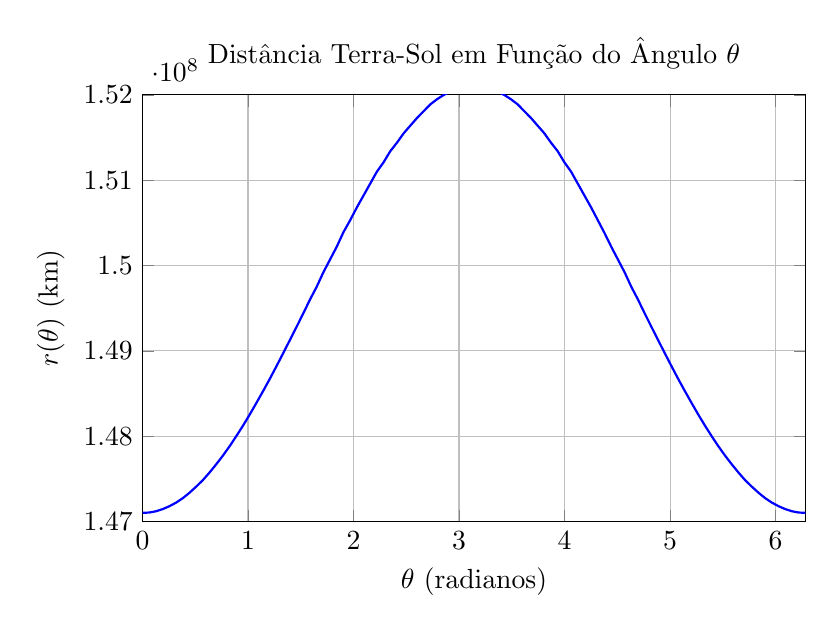
\begin{tikzpicture}
			\begin{axis}[
				xlabel={$\theta$ (radianos)},
				ylabel={$r(\theta)$ (km)},
				title={Distância Terra-Sol em Função do Ângulo $\theta$},
				xmin=0, xmax=2*pi,
				ymin=1.47e8, ymax=1.52e8,
				grid=major,
				width=10cm,
				height=7cm,
				]
				\addplot[
				domain=0:2*pi,
				samples=100,
				thick,
				blue,
				]{1.496e8 * (1 - 0.0167^2) / (1 + 0.0167 * cos(deg(x)))};
			\end{axis}
		\end{tikzpicture}
	\end{center}
	
\end{document}
